\documentclass[12pt]{article}

% House style preamble
\input{.house-style/preamble.tex}

% Update PDF metadata
\hypersetup{
  pdfauthor={},
  pdftitle={Effective without warrant: Causal-normative networks and the social life of status},
  pdfkeywords={social ontology, social kinds, projectibility, causal-normative networks, recognition, discrimination}
}
\AtBeginBibliography{\emergencystretch=3em\sloppy}

% WORKING SUBMISSION TITLE. Earlier candidates remain in planning/brief.md:
%   - What Is a Causal-Normative Network?            (blunt)
%   - Normative Status in Causal Networks            (journal-friendly)
%   - How Normative Status Enters Causal Explanation (journal-friendly)
%   - Mixed Networks: Causation, Recognition, and Deontic Status
%   - The Structure of Causal-Normative Explanation
\title{Effective without warrant: Causal-normative networks and the social life of status}
\author{}
\date{}

% Typed-edge network diagrams (local figure support)
\usepackage{tikz}
\usepackage{float}
\usetikzlibrary{arrows.meta, positioning}
\definecolor{xGreen}{RGB}{27,158,119}
\definecolor{xOrange}{RGB}{217,95,2}
\definecolor{xPurple}{RGB}{117,112,179}
\tikzset{
  kind/.style={draw, rounded corners, align=center, font=\small, inner sep=3pt, minimum height=9mm},
  ghost/.style={draw, rounded corners, align=center, font=\small, inner sep=3pt, minimum height=9mm,
                draw=gray, text=gray, dash pattern=on 2pt off 1.5pt},
  flagged/.style={draw, rounded corners, align=center, font=\small, inner sep=3pt, minimum height=9mm,
                draw=black, text=black, dash pattern=on 3pt off 2pt},
  causal/.style={-{Stealth}, semithick},
  ntrans/.style={-{Triangle}, semithick, xOrange},
  constit/.style={xPurple, very thick, double, double distance=1pt},
  recog/.style={-{Stealth}, semithick, dashed, xGreen},
  void/.style={gray, very thick, double, double distance=1pt, dash pattern=on 2pt off 2pt},
}
\newcommand{\edgelegend}{%
  \begin{scope}[shift={(0,-1.6)}]
    \draw[causal] (0,0) -- ++(0.9,0);    \node[right,font=\footnotesize] at (1.0,0) {causal};
    \draw[constit] (0,-0.6) -- ++(0.9,0); \node[right,font=\footnotesize] at (1.0,-0.6) {correlative};
    \draw[ntrans] (5.2,0) -- ++(0.9,0);   \node[right,font=\footnotesize] at (6.2,0) {status-transition};
    \draw[recog] (5.2,-0.6) -- ++(0.9,0); \node[right,font=\footnotesize] at (6.2,-0.6) {recognitional};
  \end{scope}%
}

\begin{document}
\maketitle

\begin{abstract}
Social explanation faces a forced choice: treat social statuses as causal patterns with moral labels, or as normative facts whose social uptake is incidental. Neither fits a person effectively hounded for a promise they never made, or a standing that a practice successfully confers while morality rejects it. Status-assignments, I argue, are projectible: observing one licenses defeasible expectations about duty, recognition, and response. From a promise we project duty and reliance; from release, lapse even while demand continues; from judgment, records, enforceability, and preclusion; from discriminatory standing, credibility loss, exclusion, and anticipatory adjustment. Extending \textcite{khalidi2018nodes} on projectible kinds, I model these projections as travelling through a \term{causal-normative network}: a typed structure joining causal uptake, recognitional representation, directed status-transition, and non-directed correlative ties within a practice or field. Interventionist tests type the edges, and misrecognition supplies the diagnostic case: the framework separates what a false recognition can still cause from what a wrongfully conferred standing has become. The payoff is an account of how status-assignments can be socially effective, institutionally valid or communally conferred, enforceable or final, recognitionally mistaken, and morally unwarranted in different combinations.
\end{abstract}

\noindent\textbf{Keywords:} social ontology, social kinds, projectibility, causal-normative networks, recognition, discrimination.

\section{The problem of mixed explanation}
\label{sec:problem}

Dickens gives the problem its comic legal form in \emph{Bardell v. Pickwick}: a misconstrued exchange becomes an action for breach of promise, then a damages verdict, and then Fleet Prison.\footnote{In \emph{The Pickwick Papers}, Mrs Bardell's action lays damages at \pounds 1,500, the jury awards \pounds 750, and Pickwick's refusal to pay carries him toward imprisonment for debt \citep[chaps.~26, 34, 40--41]{dickens1837PickwickPapers}.} Put abstractly, suppose a community or court comes to treat someone as having promised when he hasn't, or as bound by a debt he never incurred.

The treatment isn't imaginary: he's asked to pay, blamed when he refuses, distrusted, perhaps shut out. But if the promise was never made, those responses lack the obligation they purport to answer to; the demand has the social force of a warranted demand without its warrant.

Cases of this sort generalize: some social statuses are real in their effects without being morally warranted; some are institutionally valid (the paperwork is in order), or successfully conferred by a communal practice (imposed by agents with the social standing to make it stick), and still unwarranted. The problem is to explain what can be projected from such assignments (what observing the assignment licenses us to defeasibly expect about further status, recognition, and response; \cite{Goodman1955}), and why those projections don't settle warrant.

One reduction identifies the status with the treatment: being a debtor just is being treated as one. On that view, the wrongly-hounded man is indistinguishable from a genuine debtor, because the treatment is the same in both cases. The other reduction treats the status as only a rule-bound normative fact: whether he owes turns on whether a promise was made, and on nothing else. On that view the hounding is irrelevant, but the hounding is the phenomenon that set the problem.

Much social explanation proceeds as if these two reductions exhausted the options: model such cases as a causal network with moral labels, where the labels do no explanatory work, or as a normative taxonomy with sociology appended, where the uptake explains nothing about the status. Call that assumption the \term{forced choice}. It's this paper's opponent: both layers belong in one explanatory structure, and neither reduces to the other.

Both reductions have serious backing, and the choice between them structures live debates. Audit studies treat discrimination as a causal path from signal to response \citep{bertrandMullainathan2004EmilyGreg}, and critics object that the category so treated is constituted, not merely causal \citep{kohlerHausmann2019EddieMurphy}. Hohfeldian taxonomy states deontic structure exactly and stops before uptake, the responses that act on a recognized status \citep{hohfeld1913SomeFundamental}. In social ontology the same dialectic runs between rule-based and equilibrium-based accounts of institutions \citep{hindriksGuala2015InstitutionsRulesEquilibria}, and between what grounds a status fact and what its recognition causes \citep{epstein2015AntTrap,asta2018Categories}.

The question this paper puts to that debate is what single structure lets both halves figure in one explanation without one absorbing the other.

The answer needs both layers: a normative position, and a recognitional-causal path in which recognition can fit that position or fail to fit it, while uptake follows either way. It also needs three families of assessment kept apart: social efficacy, institutional validity or communal conferral, and moral warrant.

Promising is the case I work through, because its \term{life-cycle} (the recurring sequence a promise runs from creation to discharge) is familiar and its parts are clean: an act creates an obligation, the obligation is recognized and relied on, breach sets off demand and repair, release cancels the obligation. The same shape recurs in consent, in official judgment, and, most systematically, in discrimination, where an assignment that's effective and successfully conferred within its practice hardens into a regime that morality disowns (Section~\ref{sec:misrecognition}). I keep to promising until then.

False promise and discrimination pull the model in different directions. In the false-promise case, the status fails to obtain and recognition answers to nothing. In the discriminatory case, the standing may be genuinely conferred and real while remaining unwarranted. Promising is the clean entry case, not the template for both.

The structure I defend is a \term{causal-normative network}: a directed graph whose nodes are status-relevant items, states, and events, and whose edges are relations of real dependence. The dependence comes in three types, displayed by four types of edge.

First, \term{causal production}: one event, disposition, procedure, response, record, sanction, or expectation helps produce another. A recognized promise can cause reliance; a judgment can cause enforcement; a recognition state causally drives treatment, and that uptake is where much of the network's efficacy lies.

Second, \term{recognitional representation}: a belief, record, or official classification purports to track a status, base, or finding, fitting it, misfitting it, or answering to no status at all. What recognition then drives is causal uptake: demand, sanction, reliance, exclusion.

Third, \term{status-determination}: field-grounded relations fix whether a status obtains. In the graph, this one type of dependence appears as two types of edge. A directed status-transition edge runs from a performance, rule, status, or transition event to the status it generates, blocks, terminates, defeats, or modifies. An undertaking generates a duty; release terminates it; withdrawal terminates a permission; breach changes what later demand, blame, apology, repair, or excuse would answer to.

A non-directed correlative tie links deontic positions within a single complex. A duty and the claim-right held against the duty-bearer are one jural relation under two descriptions \citep{hohfeld1913SomeFundamental}, so from either one reads off the other. The tie is correlative, not causal.

These types of dependence and the edges that display them describe the structure of the network. They don't yet say whether a status-assignment is valid. Assessment is cross-cutting. An assignment is effective when recognition and uptake fire; \term{field-valid} when it satisfies institutional rules; successfully conferred when agents with conferral standing in a communal practice (the social position to impose such statuses) place someone under constraints and enablements; and morally warranted when the standing or treatment has moral authority.

A \term{field} here is a normative practice or domain, such as ordinary promising, friendship, contract law, criminal law, or medical ethics, with its own statuses and conditions for generating them. Institutional fields fix offices, procedures, records, and rules. Communal fields fix standing relations without a single authorizing office. Section~\ref{sec:fields} treats fields as the practice-relative settings in which statuses support projections.

The network is a representation of real dependence relations: the field-relative grounds of statuses, their correlative positions, the recognitions that fit or misfit them, and the uptake that supports social projection from those statuses. In Epstein's vocabulary, a field's \term{frame principles} specify what grounds each of its statuses, and \term{anchoring} names the facts that put those frame principles in place \citep{epstein2015AntTrap}; the network explains how the conditions they fix combine with recognition and causal response.

The claim throughout is about display, not replacement. Grounding, conferral, and causal mechanism can each list their own facts; the coupled structure is what makes explicit where projections travel, where they change type, and where warrant fails to follow.

\section{Why ordinary causal networks aren't enough}
\label{sec:causal-not-enough}

One tempting simplification is to treat causal-normative networks as ordinary causal networks with moral labels added. The best reason to try that comes from \textcite{khalidi2018nodes}. Khalidi takes projectibility as the mark of a kind: if something is gold, one can infer its melting point, density, conductivity, and other properties; if something is merely dirt, the label tells us much less. A kind matters for explanation when membership supports such inferences.

For Khalidi, those inferences work because the properties are ordered, not because the same properties merely travel together. Gold's atomic structure explains many of its other properties. A directed causal graph captures that order: change one property in the right way, hold the rest fixed, and another property shifts. Khalidi's contrast case is a widget mass-produced to a blueprint at a billionaire's whim: its many shared properties are associated by fiat, a heap rather than an ordered pattern, so being a widget supports almost no projection.

Khalidi's point should be preserved: projection needs order. The question is whether all useful order in the moral and institutional domain is causal order.

Promises make the limit visible. Suppose Nora promises to return a borrowed book on Friday. From the promise we can infer several things: Owen has a claim, Nora owes performance, Owen may rely on the book's return, breach may license demand or apology.

Some of those inferences are causal projections. When Nora's words are recognized as a promise, they may cause Owen not to buy another copy. But the duty and the claim-right aren't cause and effect; they're the same promissory relation viewed from two sides, so the step from one to the other is a read-off, not a prediction.

Release makes the point again. If Owen releases Nora on Thursday, the same Friday non-return no longer counts as a breach. The release needn't cause the non-return, move the book, or change Nora's later conduct. It changes the field conditions under which the later non-performance has breach status. That dependence is directed status-determination: the release defeats the duty, and with the duty gone the same non-return is no breach. It supports projection from release to the absence of liability or repair, but it isn't causal production in Khalidi's sense.

Consent has the same shape: withdraw it before the procedure, and the incision that follows changes status, from permitted treatment to a wrong, even if no one on the ward has heard and the causal machinery keeps moving. The withdrawal orders the later facts because it changes what the later act is.

In what sense, then, are promises, consents, and judgments projectible? Not because \mention{promise} entails its consequences as a matter of definition. The projectibility claim concerns defeasible expectations: that an undertaking generated a duty (defeated by joke, coercion, or want of standing), that recognition and reliance will follow (defeated by inattention or distrust), that breach will draw demand, apology, or repair (defeated by release or excuse).

Those expectations are inductive licences of the sort Khalidi's account trades in, not deductive consequences of a label. The one strict inference in the set, from duty to correlative claim-right, is a read-off, and Section~\ref{sec:typed-edge} sets it apart from projection proper.

The extension to Khalidi is narrow. Khalidi himself treats it as a live possibility that fundamental physics tracks structural real patterns while the special sciences track causal ones \citep[pp.~211--212]{khalidi2013}. The moral and institutional cases make a parallel but more local point: some of their order is carried by status-determination and recognitional links rather than by causal mechanisms alone. Section~\ref{sec:typed-edge} builds that typed network; the point here is only that ordinary causal networks are too narrow, not that order was the wrong demand.

\section{Why normative taxonomies aren't enough}
\label{sec:normative-not-enough}

The opposite simplification keeps the normative structure and strips away the causal uptake. That's tempting too. Analytic jurisprudence has mapped much of the structure: \textcite{hohfeld1913SomeFundamental} sorts deontic positions into correlatives and opposites, claim and duty, power and liability. A taxonomy in this style can say that a promise generates an obligation, consent a permission, release a termination, and breach a license to complain.

That taxonomy is indispensable, but it's not yet an explanation of projection in practice. Suppose Nora fails to return the book. The taxonomy says she's breached and that Owen may complain. It doesn't say whether Owen notices, whether the complaint is taken up, whether Nora apologizes or offers an excuse, whether repair follows, or whether trust changes between them.

Those further regularities are what make promise-breaking projectible as a social kind. Breach has a recognizable place in a life-cycle: registration; demand; excuse or apology; repair or sanction; revised trust. The status starts the sequence, but the sequence runs through recognition and causal uptake.

Official judgment makes the same point in a more formal register. A taxonomy can say, in broad terms, that a judgment creates an adjudicated liability, a final or preclusive position, or a remedial power \citep[\S\S~17--19, 24, 27]{americanLawInstitute1982RestatementJudgments}. But what makes judgment projectible in practice is also the file, the docket entry, the enforcement routine, the attorney's letter, the threat of contempt, and the debtor's changed bargaining position. Those aren't further deontic implications written into the word \mention{judgment}; they're the ordinary uptake by which a legal status becomes socially and institutionally effective.

This is why a purely normative taxonomy is too thin. A status no one could recognize, rely on, or enforce would support no social projection at all. It'd still be a status, but it wouldn't explain the patterned responses by which promise-breaking, consent withdrawal, judgment, or discriminatory ascription become stable objects of expectation.

The two reductions now fail from opposite sides: causal order alone was too narrow; normative order alone is too thin. Since those were the forced choice's only options, the assumption fails with them. The explanatory unit is neither causal regularity nor normative status by itself, but a normative position coupled to causal uptake. Section~\ref{sec:misrecognition} turns to the cases in which the two come apart.

\section{The typed-edge model}
\label{sec:typed-edge}

If the explanatory unit couples a normative position to causal uptake, the graph has to show both parts. In the promise case it has to show the obligation and claim-right; otherwise the graph can't say whether a demand answers to an obligation or misfires. It also has to show uptake, reliance, demand, and repair; otherwise the promise has no social life.

I keep Khalidi's picture of a kind as a highly connected node in a directed graph \citep{khalidi2018nodes}, but I let the edges differ in type. The vertices are status-relevant items, states, and events; the edges are typed relations of real dependence.\footnote{Formally, this is a typed-edge relational structure: node labels for kinds, edge labels for dependence types, and well-formed configurations. \textcite{pullumRogers2008Expressive} use a similar node/edge format for English syntax; the analogy only marks the intended level of abstraction. \textcite{pullum2001} set out the model-theoretic stance.}

The graph represents real dependence relations without becoming a further social object or an added ground of the statuses it represents. Representation in this sense is the modeller's relation to the world; it's distinct from the recognitional edges inside the graph, which mark one social item, a belief or record, representing a status. Nora's duty is grounded by her undertaking under the rules of the relevant field; Owen's claim-right is the correlative position; Owen's reliance is an ordinary causal effect; his recognition is a representation of the duty.

The realism is modest: the dependence types differ in their counterfactual behaviour, and the network displays those differences together so that projections across them can be tracked.

A status-transition edge is a directed status-determination edge: under the field's frame principles, the source item is among the grounds, defeaters, or status-altering conditions for the target status. The edge displays that field-grounded relation.

The strongest rival is a division of labour: use grounding and anchoring to explain the status, then use causal mechanisms to explain uptake. That rival is right that the graph doesn't replace grounding and anchoring. It goes wrong one step later, in treating the two explanations as separate ledgers, each keeping its own books, whose combination leaves nothing further to display.

What remains is the assignment's \term{projection profile}: which inferences it supports, along which edges, with which defeaters. The same assignment can support a transition inference, a correlative read-off, a recognition inference, and an uptake inference, while failing at a different assessment point.

A release cancels the duty even if demand continues. A mistaken verdict can make enforcement and preclusion projectible without making the underlying finding true. A discriminatory standing can be successfully conferred and predict credibility loss, routing, sanction risk, and anticipatory adjustment while remaining morally unwarranted. Separate ledgers can list the facts; the diagnostic pattern remains implicit.

The discrimination case shows the gain. A false recognition and a wrongful conferral can both be effective without warrant. If the only ledgers are grounding and causation, that common structure is easy to state and the difference is easy to miss.

The false-recognition case is locally correctable: remove the mistaken recognition and the demand lapses, since there never was a status for it to answer to. The wrongful-conferral case is recursive: earlier uptake helps constitute the standing that later recognition answers to. The network earns its keep by making that difference part of the projection profile rather than an after-the-fact comparison between two explanations.

To draw such a graph, start with the explanatory question. If the question is why Owen may demand performance, the duty and claim-right matter. If the question is why Nora is shunned despite never promising, the false recognition and its causal uptake matter. If the question is why a court order leads to enforcement, the judgment and the enforcement machinery matter.

The node types are simple. Performances include utterances, signed documents, actions, and omissions. Statuses include obligation, permission, power, liability, immunity, and standing. Status-transition sources include undertaking, authorization, release, withdrawal, breach, and defeat. Recognition states include belief, record, and official classification. Uptake and response states include reliance, demand, blame, resentment, apology, repair, sanction, exclusion, and trust revision.

Not every fact in the room gets a vertex. Nora's utterance enters because it can generate the duty and become the object of recognition; the weather and the room's acoustics stay out unless the explanatory question makes them matter.

The admission rule is practical: add a node only if leaving it out would make the explanation worse. A performance enters when it can generate, alter, defeat, or causally move a status, recognition, or response. A status enters when the field's conditions make it obtain. If the dispute is whether the status obtains, as with Pickwick's alleged promise, the graph may mark the candidate as absent rather than draw it as an ordinary status node.

Now change the case. Suppose Nora never promised, but Owen misheard a joke as an undertaking. The graph shouldn't smuggle in a duty node to make sense of Owen's anger. Outrage isn't an admission rule. It should show Owen's recognition state and its causal downstream: demand, blame, distrust. The absent duty is part of the explanation, because it's why the demand misfires. A purely causal graph would see only Owen's anger; a purely normative taxonomy would see only the absence of duty. The mixed graph shows both.

The same discipline applies to edges. Draw a causal edge only where one item helps produce another. Draw a status-transition edge only where a performance, rule, status, or transition event generates, terminates, blocks, defeats, or modifies a status. Draw a correlative tie only where two positions are correlatives of a single relation. Draw a recognitional edge only where recognition fits an actual status node.

That last rule matters: in a false-promise case, demand doesn't prove a duty. The graph should show a recognition node with live causal uptake and no fitting recognitional edge to an actual duty. Nor should moral warrant appear as a further status node that causes legitimacy; warrant is an assessment of the assignment. And the duty--claim-right tie shouldn't be replaced with a causal arrow, since correlatives aren't two states linked by a mechanism.

Figure~\ref{fig:promise} draws the four edge types in the promise case. Two further notions sit just outside that inventory. One is \term{authorized recognition}, the judgment case: a court records a liability and, because the field authorizes the court to do so, creates a new procedural status.

\begin{figure}[tb]
  \centering
  \resizebox{\textwidth}{!}{%
  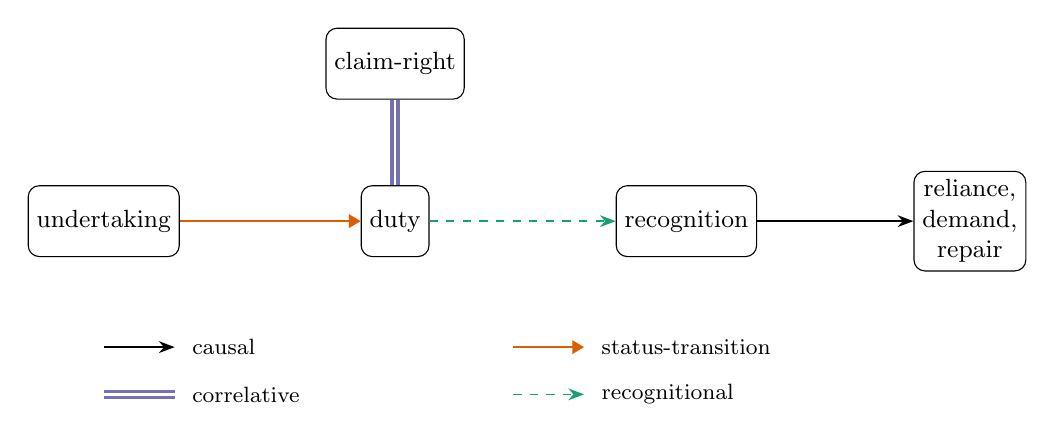
\begin{tikzpicture}
    \node[kind] (u) at (0,0)    {undertaking};
    \node[kind] (o) at (3.7,0)  {duty};
    \node[kind] (k) at (3.7,2)  {claim-right};
    \node[kind] (r) at (7.4,0)  {recognition};
    \node[kind] (d) at (11.0,0) {reliance,\\demand,\\repair};
    \draw[ntrans]  (u) -- (o);
    \draw[recog]   (o) -- (r);
    \draw[causal]  (r) -- (d);
    \draw[constit] (o) -- (k);
    \edgelegend
  \end{tikzpicture}}
  \caption{A promise as a causal-normative network. The undertaking generates the duty (a status-transition); the duty carries its correlative claim-right (a correlative tie, drawn without an arrowhead, since correlatives are one relation under two descriptions, not a directed cause); the duty is tracked by recognition, which causally drives reliance, demand, and repair. The recognitional edge is drawn from the duty node for simplicity: recognition may track the duty--claim-right complex under either description. In failed cases the recognition node remains without a fitting edge (Section~\ref{sec:typed-edge}). The four edge types are keyed below the graph.}
  \label{fig:promise}
\end{figure}

The other is \term{projection}: using one point in the network to make defeasible inferences about what else should hold or what will happen next. I restrict the term to inferences that further facts could defeat. The correlative tie licenses something stricter, a \term{read-off}: given the duty, the claim-right isn't a further expectation but the same relation redescribed. Read-offs are exact and indefeasible, so they're not projections.

Counterfactual probes help reveal the projection profile, but they don't supply a one-step classifier for every edge. I reserve \term{intervention} in the strict Woodwardian sense for causal edges. \textcite{woodward2003MakingThingsHappen} counts a relation as causal when some possible intervention on the first variable changes the second while everything else is held fixed, and the change reaches the second only through the first \citep{woodward2014MethodologyOntology}.

A causal edge passes this test in the ordinary way: intervene on the recognition state and reliance shifts (in Figure~\ref{fig:promise}, the edge from recognition to reliance, demand, and repair), intervene on the judgment and enforcement may follow. Khalidi already reads his own causal edges this way \citep{khalidi2018nodes}, which is why typing the edges extends his picture rather than breaking with it.

A correlative tie fails the test in a way that helps mark its type. A duty and its correlative claim-right (the unarrowed double tie in Figure~\ref{fig:promise}) aren't two states linked by a mechanism; they're one jural relation under two descriptions \citep{hohfeld1913SomeFundamental}. No intervention changes the duty while holding the claim-right fixed, because changing the one just is changing the other: the change doesn't reach the claim-right only through the duty, it lands on both at once. By Woodward's own criterion the tie isn't causal, and that failure is what marks it as correlative rather than causal.

Status-transition cases behave differently. Release, withdrawal, undertaking, and judgment alter the field conditions under which a status obtains; generation is Figure~\ref{fig:promise}'s undertaking-to-duty edge. Their dependence is directed, but it's directed status-determination rather than causal production: release the promisor and the same non-performance is no longer a breach. Hohfeldian correlatives are the limiting non-directed case, because duty and claim-right aren't successive statuses at all.

The positive mark of status-determination is determination rather than production: it fixes, defeats, or alters whether a status obtains, rather than pushing uptake along a mechanism. Some cases, such as duty and claim-right, also fail Woodward's distinctness condition outright. Others, such as undertaking to duty, may involve distinct relata. The type is unified not by one Woodwardian failure mode but by its role in fixing status rather than producing uptake.

A recognitional edge connects an actual status node to a recognition node that fits it (the dashed edge from duty to recognition in Figure~\ref{fig:promise}). A belief, record, or classification, itself driven by signals and cues along causal edges, may also misfit or answer to no status at all. In those failed cases the recognition node remains, with its outgoing causal edges, but the fitting recognitional edge is absent or failed. That gap is what the \mention{mis-} in misrecognition marks.

One occurrence can also enter more than one relation. The same utterance \mention{I'll do it} may generate a duty if made under the right conditions, become the object of later recognition, and support reliance through that recognition. The same court order can be evidence in one setting, an operative change in another, and the cause of enforcement in a third.

When representation succeeds, recognition tracks the status (Figure~\ref{fig:promise}). Fit is separate from downstream uptake: treatment, demand, sanction, reliance, and exclusion follow causal paths. Those paths are where a status becomes socially effective, and so where the normative layer re-enters social explanation.

\textcite{sbisa2023OnIllocutionaryTypes} describes illocutionary acts as assigning or cancelling deontic-modal predicates; on this model, such an act appears as a performance feeding a status-transition edge.


Two conditions keep such a graph from sliding back into a mere list of properties. First, inference has to respect edge type. The inferential ledger is mixed: causal edges license projections of uptake or response; status-transition edges license projections from performances or rules to generated, defeated, or altered statuses; recognitional edges license projections about tracking, misfitting, and downstream uptake; correlative ties license only read-offs, redescriptions rather than projections.

Second, a status that's meant to explain a \term{social cascade} (the run of responses in which one agent's uptake becomes the next agent's cue: demand, enforcement, apology, exclusion, repair) has to be linked to response states through recognition and causal uptake. A status can obtain without being noticed, but it explains projectible cascades only where the field supplies pathways by which agents can track or respond to it.

Table~\ref{tab:projection-ledger} gives the compact ledger for the four carrying cases: what type of inference each source item supports, and where that inference can fail.

\begin{table}[H]
\centering
\footnotesize
\setlength{\tabcolsep}{3pt}
\begin{tabular}{@{}>{\raggedright\arraybackslash}p{0.15\textwidth}>{\raggedright\arraybackslash}p{0.16\textwidth}>{\raggedright\arraybackslash}p{0.16\textwidth}>{\raggedright\arraybackslash}p{0.25\textwidth}>{\raggedright\arraybackslash}p{0.18\textwidth}@{}}
\toprule
Case and field & Source item & Main edge & Projection or read-off & Defeater or limit \\
\midrule
Promise, ordinary promising & Undertaking & Status-transition; correlative & Duty (claim-right by read-off); reliance, demand, apology, or repair if recognized & Joke, coercion, release, or lack of authority to bind \\
Consent, medical ethics & Consent or withdrawal & Status-transition; recognition-to-uptake & Permission, its lapse, charting, stopping, complaint, or apology & Incapacity, defective disclosure, withdrawal, emergency, or missed recognition \\
Judgment, law & Court judgment & Authorized recognition: recognition plus status-transition & Adjudicated status, record, finality or preclusion, remedial and enforcement position \citep[\S\S~17--19, 24, 27]{americanLawInstitute1982RestatementJudgments} & Lack of jurisdiction, appeal, reversal, procedural defect, or moral error \\
Discrimination, communal practice & Signal or ascription plus empowered uptake & Causal recognition path; communal conferral & Lowered credibility, restricted options, risk, routing, anticipatory adjustment & Weak uptake, counter-practice, lack of conferral standing, or no durable position \\
\bottomrule
\end{tabular}
\caption{A compact projection ledger. Each row gives the field, the source item from which projection starts, the main edge type, the target of projection (with read-offs marked), and the defeaters or limits that keep projection from becoming moral warrant.}
\label{tab:projection-ledger}
\end{table}

With those conditions in place the graph carries order in Khalidi's sense, projection along directed edges, while generalizing what that order is: not causal dependence throughout, but causal, recognitional, and status-determination routes. The non-directed correlative tie is the limiting case, licensing read-offs rather than projections.

All these nodes and edges are field-indexed. Contract law, medical ethics, friendship, and discriminatory practices fix different repertoires, authorities, records, responses, and defeaters; Section~\ref{sec:fields} returns to the field parameter.

\section{Coupling and counterfactual patterns}
\label{sec:coupling}

The easiest way to see the coupling is to ask simple what-if questions. What if Owen releases Nora? What if Owen mistakenly believes Nora promised? What if a court enters judgment? Each change moves a different part of the graph, and the pattern tells us which type of edge is doing the work. I call these \term{counterfactual patterns}.

The first what-if changes a status or the rule behind it. Release the promisor and later non-performance is no longer a breach; the demand, blame, and repair that breach would license lapse because the breach status is gone. Withdraw consent and the same act of touching changes from permitted to wrongful. Speak without standing and the same words fail to bind; an official's words and a bystander's words don't have the same status effects. These are the status-altering acts the normative-powers literature describes \citep{owens2012ShapingNormativeLandscape,raz2022NormativePowers}.

Call that a \term{status-rule pattern}. The status node changes first in the order of explanation, and uptake follows because agents now have a different status to recognize or answer to. The audience may be psychologically unchanged at the first moment: Owen may still expect the book, the doctor may still prepare the procedure, the clerk may still open the file. What's changed is what their responses would now be responses to. The pattern licenses projection from release, withdrawal, or authorization to changed duty, permission, liability, or remedial position even when uptake lags.

The consent example is useful because the surface behavior can remain almost unchanged. A clinician reaches for the same instrument, at the same time, for the same medical reason. Before withdrawal, the permission licenses that act. After withdrawal, the same act of touching is no longer licensed. If the clinician hasn't heard the withdrawal, her recognition node may still represent the old permission, and her action may continue along the old causal path. The status-rule pattern and the recognition pattern come apart in one ordinary case.

The second what-if changes recognition while the status stays put. Return to the misheard joke: Nora never promised, but Owen and the audience believe she did. There's no promise-duty node for recognition to fit, but the false recognition node can still drive demand, blame, and loss of trust. Suppose consent has been withdrawn but the withdrawal isn't registered. The permission has lapsed, but the old response path may keep running.

Call this a \term{recognition pattern}: whether the recognition fits the status, misfits it, or answers to nothing, the causal edge leaving it can fire.

In hiring, changing the employer's belief about an applicant's gender changes the recognition node and the causal edge from recognition to callback while leaving the applicant and the moral facts unchanged. Woodward's own reading of \mention{being a woman causes hiring discrimination} relocates the cause to the employer's beliefs about the applicant's gender \citep{woodward2014MethodologyOntology}. That's a recognition pattern in this sense: it projects efficacy without projecting warrant.

The third what-if is the compound case. A judgment records, finds, or accepts a status, but the field also gives the judgment a power to change the parties' statuses. Before judgment, the alleged liability may be disputed. After judgment, the field may treat the parties as occupying a new procedural or remedial position even where the court is mistaken: a record, enforceability, finality or preclusion, or remedial power \citep[\S\S~17--19, 24, 27]{americanLawInstitute1982RestatementJudgments}.

Contract law has parallel discharge devices, such as accord and satisfaction or a contract not to sue, that alter the obligation itself even if demand continues \citep[\S\S~281, 285]{americanLawInstitute1981RestatementContracts}.

The compound case is \term{authorized recognition}. Authorized recognition isn't a fifth primitive. The same judgment-node occupies two roles: recognition, because the judgment records or finds; transition, because the field authorizes that recognition to make a status difference. The pattern projects field-valid procedural consequences from the authorized act without projecting moral warrant or truth of the underlying finding.

Pickwick again shows why the compound matters. The alleged proposal doesn't by itself create the promised obligation. But the verdict creates an adjudicated liability within the procedure of the court. That position can be entered in a record, treated as settled for procedural purposes, and routed into remedial or enforcement machinery. One mistake is to say that the judgment merely recognizes a liability already there. Another is to say that the judgment is just a cause of imprisonment. It's both recognition and status-transition: a finding that the field treats as operative.

\textcite{pearl2009} distinguishes three levels of causal question: association asks what accompanies what, intervention asks what would follow if a node were set by fiat, and counterfactuals ask what would have held had things gone otherwise. The what-if patterns above are questions of the second and third levels, but only the causal edges answer to the do-operator, Pearl's formal device for setting a node by fiat; on transition and correlative structure, the answers are fixed by the field's rules rather than by mechanisms.

These patterns depend on a separability assumption. We have to be able, at least in explanation, to change one node or edge while holding the adjacent structure fixed. Woodward calls this \term{modularity}: mechanisms are separately disruptable in principle \citep{woodward2003MakingThingsHappen}. The condition isn't trivial. In an actual field, rules, records, and uptake often move together, which is why the patterns are explanatory probes rather than field experiments. If a public release also changes belief, the graph records both a status-rule change and a causal update in recognition.

That qualification matters most in communal-conferral fields. In promising, consent, and formal judgment, one can often hold status fixed while varying recognition, or hold recognition fixed while varying status. In conferralist cases, enough change in recognition and uptake can itself change the standing. The framework predicts partial separability there: the pathway can be probed before it hardens into a position (Section~\ref{sec:misrecognition} develops this as stage-relative).

Correlative ties fail the separability condition outright: changing the duty just is changing the claim-right. In clean cases, the status-rule and recognition contrasts can still be drawn. Release the promisor and the obligation lapses while the audience's belief can remain; change an employer's belief while the applicant's status remains. The modularity contrast helps locate causal routes and the limiting correlative cases; the remaining work is done by the field-grounded status-determination relation itself.

I set aside a pure causal intervention, such as severing an uptake mechanism so that Owen's letter of demand never arrives, because both reductive views already grant it. It can't distinguish the reductive views from the coupled account. A lost letter is too easy; the problem is a live demand with no warrant.

The status-rule and recognition patterns expose the mistake in the forced choice. The recognition reduction predicts that enough uptake turns the recognition node into the status node. The normative reduction keeps the status node but treats misfiring recognition and its causal effects as noise. The two probes show why both are wrong: demand and duty can vary separately, and the coupled, typed structure predicts which part of the case moves and which holds fixed.

An interventionist objection presses from the other direction. Why not drop the network label and disambiguate everything into manipulations of beliefs, records, and behavior? The reply turns on Woodward's own view that interventionism is methodology, not ontology \citep{woodward2014MethodologyOntology}. It clarifies causal claims by tying them to hypothetical experiments; it doesn't say that every relation clarified in that way is causal. Both probes above need the status node: without it, one can record who demanded what, but not whether the demand fitted an obligation. The disambiguation is useful, but it marks rather than removes the place where a normative edge is needed.

\section{Misrecognition as the diagnostic case}
\label{sec:misrecognition}

Misrecognition is the sharpest diagnostic because it asks a plain question: what should we say when people treat someone as bound, liable, authorized, dangerous, or disqualified, and that treatment is wrong? A recognition-only account says the treatment makes the status. A purely normative account says the treatment is noise around the real status. Neither answer fits Pickwick, who's effectively hounded as a promisor without having made the promise.

The network separates four questions. Is the assignment socially effective (do people rely on it, demand, enforce, exclude, record, sanction)? Is it institutionally field-valid (the right party, office, procedure, form, record, rule, authority)? Is it successfully conferred in a communal practice (conferral standing in context, imposed constraints and enablements)? Is it morally warranted (moral authority rather than unjust constraint)?

I offer no first-order theory of moral warrant here. Nor is warrant just field-validity in a moral field: a field supplies the practice-relative machinery (statuses, moves, records, defeaters) that makes projections usable inside it, while moral warrant is the standpoint from which those rules and conferrals are themselves answerable. That standpoint may be theorized in different moral vocabularies. Whatever supplies the standard, the warrant question asks whether an assignment has authority, and efficacy, field-validity, and successful conferral don't settle that by themselves.

Table~\ref{tab:assessment} sets out those questions, one assessment per row, with what answering each one does not settle. Some assessments are basic families; others are refinements needed for institutional, procedural, and recognitional cases. They often travel together in ordinary cases, but none carries the others with it.

\begin{table}[H]
\centering
\small
\setlength{\tabcolsep}{3pt}
\begin{tabular}{@{}>{\raggedright\arraybackslash}p{0.22\textwidth}>{\raggedright\arraybackslash}p{0.43\textwidth}>{\raggedright\arraybackslash}p{0.25\textwidth}@{}}
\toprule
Assessment & Question & Does not settle \\
\midrule
Social efficacy & Do recognition and uptake produce reliance, demand, enforcement, exclusion, records, or sanction? & Whether the status obtains or is warranted \\
Institutional field-validity & Did the right office, procedure, form, record, rule, or authority assign the status? & Truth, justice, or current recognition \\
Communal successful conferral & Did agents with conferral standing in context place someone under constraints and enablements? & Moral authority or institutional legality \\
Recognitional fit & Does the belief, record, or classification track the status, base, or finding it purports to track? & Efficacy, validity, or warrant \\
Enforceability or finality & Can the field's machinery act on the assignment, or treat it as settled for procedural purposes? & Moral warrant or underlying truth \\
Moral warrant & Does the standing or treatment have moral authority and avoid unjust constraint? & Social efficacy or field-validity \\
\bottomrule
\end{tabular}
\caption{Six assessments of a status-assignment, one per row. They often travel together, but none entails the others.}
\label{tab:assessment}
\end{table}

In a straightforward case, the assessments line up: a genuine promise may be recognized, valid in the relevant practice, and morally binding. They come apart in the hard cases. In the false-promise case, social efficacy is present if people demand and blame, but field-validity and moral warrant are absent if no undertaking occurred. In the mistaken-judgment case, efficacy is present and legal field-validity may also be present, even though the underlying finding is wrong. In the discrimination case, a community may confer a degraded standing that's socially real and stabilized by the practice, while moral warrant remains absent.

Four failure modes follow. In \term{false recognition}, uptake outruns status. In \term{wrongful institutional validity}, field rules assign the status and field-validity outruns warrant. In \term{wrongful communal conferral}, conferral standing outruns moral authority. In \term{suppressed entitlement}, the field refuses to register a moral basis: warrant outruns recognition.

Pickwick keeps the first failure mode clean: until judgment enters, there's no promised obligation for recognition to fit, and the verdict (Section~\ref{sec:coupling}) then creates a new legal liability. The episode shows efficacy without the promised obligation, not yet the regime structure of wrongful conferral.

Suppressed entitlement is the mirror image. A friend may be owed an apology, a patient may have withdrawn consent, or a party may have a procedural entitlement, while the local practice refuses to record the claim, routes around it, or treats assertion as troublemaking. The status isn't created by recognition; recognition is missing where the status should be tracked.

Regime cases require more than one mistaken uptake. A person wrongly believed to have promised faces a local failure: demand, blame, and distrust may be real, but the error can in principle be corrected by showing that no promise was made. A durable discriminatory practice is different. It repeats the ascription, routes it through records and expectations, and gives people real constraints and enablements under that description.

Ásta's conferralist account helps specify that second structure. A social status is conferred on a person because agents with conferral standing in a context take them to have some base property, whether or not they actually have it, and impose real constraints and enablements on what they may do \citep{asta2018Categories}. The ascribed standing isn't a mere belief. It's a social position with teeth.

Conferralism might seem to collapse the distinction between successful conferral and moral warrant. If the status just is what gets conferred, then enough recognition constitutes the status. But the collapse is avoided once the assessment questions are separated. Conferral can make a communal status real and effective without making it morally warranted. A discriminatory standing can be successfully conferred, stabilized by its practice, and morally indefensible at the same time.

\textcite{jenkins2020OnticInjustice,jenkins2023OntologyOppression} calls this family of wrongs \term{ontic injustice}: a person is wronged by being socially constructed as a member of a social kind when that construction places them under wrongful constraints and enablements.

On the taxonomy used here, ontic injustice spans wrongful institutional validity and wrongful communal conferral: the status may be institutionally valid without warrant, or it may be communally conferred without moral authority. Jenkins gives the moral-ontological diagnosis; the typed-edge account adds the projection map by separating recognitional classification, causal uptake, status-determination, field-validity or successful conferral, and moral warrant. That separation lets these wrongs be distinguished from false recognition and suppressed entitlement.

Some oppression works through this route: morally indefensible status-ascriptions become socially effective, and sometimes institutionally valid or successfully conferred, along durable recognition and response pathways. Not all oppression does. Much is material, distributive, or coercive rather than recognitional, as the redistribution-versus-recognition debate insists \citep{fraserHonneth2003Redistribution}. Stabilized wrongful conferral is only the case this account is built to diagnose.

Material and distributive structures aren't therefore invisible to the network. They can enter as causal constraints, resources, built environments, or enforcement routines. What this section adds is narrower: when those pathways also impose a standing, the explanation needs a status node as well as causal paths to harm.

\begin{figure}[H]
  \centering
  \resizebox{\textwidth}{!}{%
  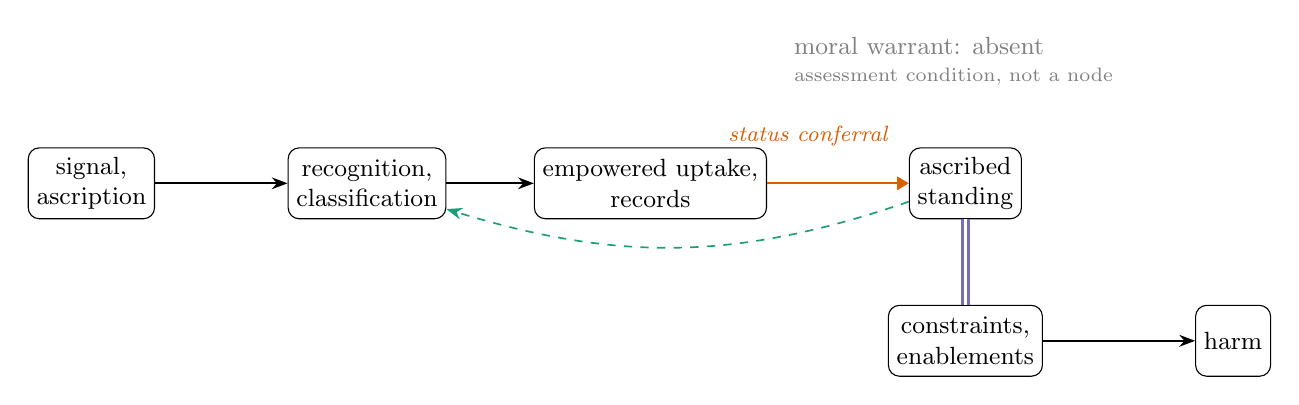
\begin{tikzpicture}
    \node[kind]    (u) at (0,0)    {signal,\\ascription};
    \node[kind]    (r) at (3.5,0)  {recognition,\\classification};
    \node[kind]    (p) at (7.1,0)  {empowered uptake,\\records};
    \node[kind]    (s) at (11.1,0) {ascribed\\standing};
    \node[kind]    (c) at (11.1,-2) {constraints,\\enablements};
    \node[kind]    (h) at (14.5,-2) {harm};
    \node[font=\small, align=left, text=gray, anchor=west] at (8.8,1.55)
      {moral warrant: absent\\[-1pt]\scriptsize assessment condition, not a node};
    \draw[causal] (u) -- (r);
    \draw[causal] (r) -- (p);
    \draw[ntrans] (p) -- (s);
    \draw[constit] (s) -- (c);
    \draw[causal] (c) -- (h);
    \draw[recog]  (s) to[bend left=18] (r);
    \node[font=\footnotesize\itshape, xOrange, anchor=south] at (9.1,0.35) {status conferral};
  \end{tikzpicture}}
  \caption{Wrongful conferral. A signal or ascription moves recognition, and recognition moves structurally empowered uptake and records. The orange edge marks status-conferral: agents with conferral standing can stabilize that uptake and confer an ascribed standing. The green dashed edge marks later recognition tracking the standing, not the conferral itself. Moral warrant, not the standing, is absent (grey annotation). This isn't the false-promise case, where recognition fails to fit an absent status. Edge styles as in Figure~\ref{fig:promise}.}
  \label{fig:misrecognition}
\end{figure}

Read Figure~\ref{fig:misrecognition} from left to right. A signal or ascription moves recognition, and recognition moves structurally empowered uptake and records. When that uptake becomes a durable practice, it can help confer a standing. The standing node isn't a hidden essence behind those patterns: it's constituted by the stabilized constraints and enablements, and it supports projections of restricted options, lowered credibility, sanction risk, anticipatory adjustment, and downstream harm.

The conferring agents are those whose uptake is structurally empowered in that context: gatekeepers, officials, employers, teachers, clinicians, peers, or a dominant local audience. The base or ascription is the property they take the person to have. The conferred status is a role-like standing in that setting rather than the base property itself: lowered credibility, suspected dangerousness, reduced authority, or disfavoured applicant standing.

Discrimination, where it runs through conferred standing, is the regime case for this account. The efficacy is measurable, if crudely. In the correspondence study by \textcite[997--998]{bertrandMullainathan2004EmilyGreg}, otherwise-matched resumes with White-sounding names drew about 50\% more callbacks than those with African-American-sounding names (9.65\% against 6.45\%), and \textcite{ayres1991FairDriving} found parallel differential treatment in retail car negotiations.

These studies show patterned uptake: a name or other raced signifier sends a causal edge to a recognition node, and that recognition node sends causal edges to callbacks, prices, warnings, searches, or other outcomes. They evidence a signal-recognition-response pathway; they don't by themselves establish a degraded standing. A normative taxonomy with no place for this efficacy can't describe what's happening.

The studies don't manipulate race itself. As \textcite{weinbergerSignalManipulation} observes, they manipulate a signal for race: the name matters because it reliably tracks race, and the experiment varies the signal to mimic what it'd be were the candidate of another race, leaving the candidate's race untouched. That's a localized causal test of the signal-recognition-response pathway. It doesn't make race an ordinary manipulable cause, and it doesn't reduce race to its signals.

Detection is still not an account of discrimination. \textcite{kohlerHausmann2019EddieMurphy} is right that a signal test can show race made a difference without saying what race is or why discriminating on it's wrong. \textcite{huForthcomingNormativeFactsCausalStructure} presses further: deciding which differences between two candidates constitute rather than confound the effect of race already takes a normative stand, so even the measurement presupposes the normative layer.

What turns biased uptake into conferred standing is entrenchment under agents with conferral standing in that context. A single misfiring is false recognition. A stable recognition-response pathway is different. When the pathway is repeated, recorded, expected, and treated as a guide for action, the entrenched pathway shapes what one may do, where, with what credibility, and at what risk \citep{asta2018Categories}. That imposed structure, not the bare frequency of mistreatment, is the degraded standing.

The contrast is between an episode and a position. A single employer's biased callback decision is an episode of differential treatment. It may be wrongful, and it may reveal a causal pathway from signal to recognition to response. A standing emerges when decisions of that sort become mutually reinforcing: employers expect other employers to read the signal the same way, applicants adjust their applications in anticipation, institutions record and route outcomes accordingly, and the burden becomes part of what one has to navigate. The graph then has a stable ascribed-standing node, not just repeated arrows from signal to harm.

The difference isn't frequency by itself: repeated false recognitions remain false recognition if each episode has to do the whole explanatory work again. A position emerges when earlier uptake becomes part of the practical background for later uptake. At that point the pathway is recursive: recognition causes treatment, treatment stabilizes expectations and records, and those stabilized expectations and records help fix the standing to which later recognition responds.

This is why separability is stage-relative. At the episode stage, one can probe the pathway from signal to recognition to response while holding standing fixed or absent. At the regime stage, that probe no longer cleanly separates standing from uptake, because the stabilized pathway has become one of the standing's conferral conditions.

The loss of clean separability isn't a collapse of the distinction between false recognition and wrongful conferral. It's the mark that the case has moved from an episode to a position. The boundary is vague, but it's not unconstrained: a standing node is warranted only when the practice supports projections that no single episode supports.

There's no sharp threshold at which episodes become a position. The standing node marks a cluster stabilized by the mechanisms already named. Borderline cases are expected. Their vagueness is the ordinary vagueness of cluster kinds, not a missing necessary and sufficient condition.

Uptake need not be endorsement. Pickwick could have paid the judgment while still denying the promise; an applicant can tailor a resume to a gatekeeper's expectations while rejecting the standing the tailoring anticipates. Strategic compliance reproduces the practice's efficacy, and some of the uptake that stabilizes a standing comes from its targets, but none of it confers moral warrant.

The failure modes also sort the remedies. False recognition calls for corrected recognition: show the promise was never made. Wrongful institutional validity calls for rule change or appeal, and suppressed entitlement for registration. Wrongful conferral is the hard case: the stabilized pathway is among the standing's conferral conditions, so correcting beliefs isn't enough, and the remedy has to de-entrench the pathway itself, deliberately bringing about the decay that overtakes any status when its uptake stops. That's why a wrongful standing can outlive the beliefs that built it.

The discrimination this account captures is entrenched wrongful conferral: recognitional and causal paths become entrenched through those mechanisms and support projection from ascription to degraded standing. Other discrimination (resource allocation, exclusionary design, statistical sorting) can wrong without conferring a degraded status; this account claims only the conferral-based cases.

\textcite[pp.~19--23]{marques2017CausalSocialConstruction} argues that causal social construction remains politically relevant even where constitutive construction is granted or unsettled. The graph should keep ordinary causal routes to harm visible alongside the narrower conferral pattern.

Wrongful conferral, then, begins where the recognition pattern of Section~\ref{sec:coupling} ends: entrench the pathway, and it helps generate a standing rather than merely misrecognizing one. Only a coupled, typed structure registers both moments: an effective recognition, and a stabilized standing without warrant.

\section{Fields}
\label{sec:fields}

A field tells the graph what counts. In contract law it tells us which words, signatures, consideration, defects, and discharge agreements generate or defeat liability \citep[\S\S~281, 285]{americanLawInstitute1981RestatementContracts}. In medicine it tells us who may consent, who may diagnose, which records count, and which responses follow. In friendship it tells us when a betrayal licenses resentment, apology, repair, or distrust.

Projectibility is field-relative in this sense. A status supports the projections licensed by the practice in which it figures. Breach in contract law projects toward liability, remedies, defenses, and excuses; in friendship, toward resentment and repair. Consent in medical ethics projects toward permission, disclosure duties, withdrawal conditions, and recordkeeping.

Discriminatory standing projects toward lowered credibility, restricted options, sanction risk, anticipatory adjustment, and institutional routing. This is close to Boyd's accommodation thought \citep{boyd1999}: a practice-relative grouping earns its keep by helping the practice make the inferences it needs, not by having sharp boundaries independent of every practice.

Epstein's frame principles and anchors (Section~\ref{sec:problem}) apply field by field \citep{epstein2015AntTrap}: the field fixes which performances ground which statuses, which records preserve those statuses, which recognitions can alter those statuses, and which defeaters block those statuses.

Those conditions don't hang together by accident. Records, registers, monitoring, enforcement routines, reputational sanction, professional training, and habituated uptake help anchor and stabilize them. A field needn't itself be a natural kind. For present purposes, stability means recurrence across cases, recognized routes for record or uptake, socially intelligible defeaters, and enough continuity that source nodes license defeasible expectations about target statuses and responses.

So the parameter is constrained. Not every useful redescription counts as a field, and not every labelled condition counts as a status: the framework misfires if the alleged field has no stabilized repertoire of moves, statuses, authorities or standing relations, record or uptake routes, and socially intelligible defeaters, or if the alleged status licenses no projections beyond the case at hand.

Nor may the field parameter be adjusted after the fact merely to save a preferred verdict: changing the field changes the projected routes and defeaters, and those changes have to be supported by the practice's rules, records, uptake, or standing relations.

Field-validity isn't the same as current recognition, enforceability, finality, or moral warrant: a contract can be valid even if a particular audience misses it. The field fixes the validity conditions; recognition is one route by which agents track or fail to track those conditions.

\textcite[pp.~6--8]{almang2016LegalFacts} makes the legal version explicit: institutional status, deontic relation, and institutional function can come apart, so status and the exercise of its normally attached function should be represented separately.

A limited analogy comes from educational measurement. \textcite{messick1995Validity} argues that validity attaches to supported interpretations and actions based on scores, not to an instrument considered in isolation. The present issue is practice-relative status validity, not measurement validity.

Communal cases need a further caution. In friendship, workplace standing, or discriminatory social position, there may be no office or rulebook that settles validity. The stricter question is whether the standing has been successfully conferred: whether agents with conferral standing in that context have imposed real constraints and enablements through a recurring practice.

This also explains why fields can be fuzzy or contested without becoming useless. A counter-practice may reject an official rule without leaving the domain altogether. Oppressive and resistant uptake can coexist in the same workplace, clinic, court, or community. The question is whether the practice has enough recurrence, record or uptake routes, and socially intelligible defeaters to fix the status conditions relevant to the projection at issue.

The field, then, parameterizes the network rather than sitting inside it as another node, fixing everything from the status repertoire to the defeaters.

Field-parameterization lets the account steer between universalism and relativism: one shared typed network, many field-specific parameterizations. \mention{Field} isn't Bourdieu's technical term here. The paper needs only a modest point, not a general sociology of fields: status facts are assessed only relative to a practice whose status conditions are stabilized well enough to support projection.

Fields come in at least two types. Institutional fields assign status functions by authorized conferral; \textcite{searle1995Construction} builds such status functions from the assignment of function, collective intentionality, and constitutive rules. A contract, diagnosis, judgment, or accepted resignation lives here, and so does authorized recognition. Speech-act practice also belongs here when an illocutionary act alters the deontic-modal position of participants \citep{sbisa2023OnIllocutionaryTypes}.

Communal fields work differently. \textcite{asta2018Categories} marks out statuses, gender and race among them, conferred by a community with conferral standing but no single office. That distinction explains why official judgment and discrimination, though both turn on recognition, behave so differently. The first is institutional: a recognition the field authorizes to make the status it records. The second is communal: a diffuse conferral with real constraints and enablements but no authorizing office. With no office to certify the conferral, standing to confer and moral authority to confer come apart directly.

\textcite[pp.~42--43]{behrensen2018MakingUpPeoples} uses the same contrast for nationality: legal nationality is conferred through administrative acts, while social nationality is a multipolar process with no central authority. The example supports the field contrast without making nationality the template for every communal conferral.

Ordinary promising and friendship are communal in this broad sense, though less regime-like than discriminatory standing. They lack a central office, but they still fix who can undertake, release, resent, apologize, repair, or defeat a claim well enough to support projection.

\section{Conclusion}
\label{sec:conclusion}

The paper began with cases in which a person is treated as occupying a status they don't have, or is assigned a standing that a practice successfully confers while morality rejects the standing. A causal graph can track the hounding, sanction, or exclusion, but not why the treatment fails to fit. A normative taxonomy can state the duty, permission, or standing, but not which social cascade that status will support. The forced choice between those two models was the opponent throughout.

Khalidi's causal-network account of kinds should be kept. Projection needs order, not concatenation. The moral and institutional cases show that the order can be carried by non-causal edges and still support projection. A causal-normative network is the typed structure, stabilized by field practices, that makes a status usable for inference.

A causal-normative network lets us project different things from the same assignment. From a release we project the lapse of obligation, even if demand continues. From a judgment we project records, enforceability, finality or preclusive effects, and remedial powers, while leaving truth and warrant open. From a discriminatory standing we project credibility loss, constrained options, sanction risk, institutional routing, and self-adjustment, while withholding moral warrant.

The framework does more than remind us that some explanations contain both causal and normative material. Its stronger claim concerns the shape of the projection profile. Separate explanations may remain true; the assignment's projection profile is still a mixed object. The profile becomes explicit only when causal, recognitional, and status-determination routes are displayed together, with status-determination split between directed transitions and non-directed correlatives. That's why false recognition, wrongful institutional validity, wrongful communal conferral, and suppressed entitlement can be compared across fields.

It's part of the claim to say what would count against it. If every diagnosis here restates without loss in the separate vocabularies of grounding, conferral, and causal modelling, the network is idle, and for a framework idleness is failure. If transition-inferences are rule-application in disguise, so that conditionalizing on their defeaters leaves nothing defeasible, the status-transition route collapses into read-off. If no entrenched practice supports projections beyond what its episodes supply, wrongful conferral collapses into repeated false recognition. The account stands with these commitments.

The model earns its keep by letting us compare such cases without flattening their edge types into one, and distinguish their failure modes without isolating status from uptake.

\section*{Statements and declarations}

The author has no relevant financial or non-financial interests to disclose. The large language models Claude and ChatGPT served as drafting and editing aids in the preparation of this paper, beyond AI-assisted copy editing; the author is responsible for all theoretical claims, arguments, errors, and interpretive choices.

\newpage
\printbibliography

\end{document}
